\begin{frame}[fragile]
\secframetitle{\ssCharm}
%--------------------------------------------------
\framesubtitle{\charm\ parallel programs: collections of asynchronously-interacting objects}
%--------------------------------------------------
\begin{minipage}[t]{1.75in}
\begin{center}
\begin{minipage}{1.25in}
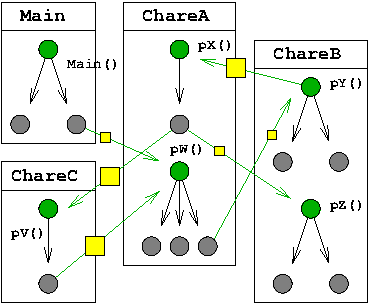
\includegraphics[width=1.25in]{charm.pdf}
\ \\
\centerline{\scriptsize\textbf{A Charm\pp\ parallel program}}
\end{minipage}\\ \ \\
\ \\
\hrule
\ \\
\begin{minipage}{1.50in}
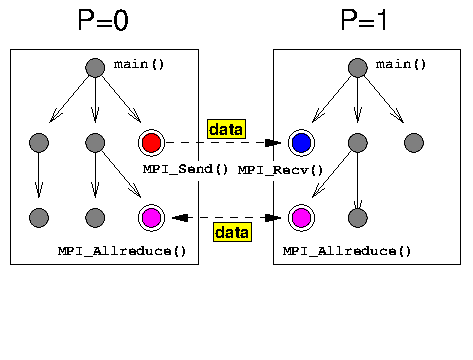
\includegraphics[width=1.50in]{mpi.pdf}\\
\vspace{-0.5in}
\centerline{\scriptsize{An MPI parallel program}}
\end{minipage}
\end{center}
\end{minipage} \ 
\begin{minipage}[t]{2.50in}
\vspace{-0.70in}
\begin{itemize}
\item \charm\ program
  \begin{itemize}
  \item Decomposed by \blueit{objects}
  \item \charm\ objects called \blueit{chares}
  \item invoke \blueit{entry methods}
  \item \blueit{asynchronous}
  \item communicate via \blueit{messages}
  \end{itemize}
\ \\ \pause
\item \charm\ runtime system
  \begin{itemize}
  \item maps chares to processors
  \item schedules entry methods
  \item migrates chares to load balance
  \end{itemize} \pause
\item Additional features
\begin{itemize}
\item checkpoint/restart
\item dynamic load balancing
\item fault-tolerance
\end{itemize}
\end{itemize}
\end{minipage}
\end{frame}
